\documentclass{article}
 % Add your name here
\usepackage{graphicx} % Required for inserting images
\usepackage{amsmath}
\usepackage{amssymb}
\usepackage{floatrow}
\usepackage{changepage}
\title{EE338 : Digital Signal Processing \\ Chebyschev Filter Design Assignment}
\date{}

\begin{document}

\maketitle

\section{\textbf{Student Details}}
\textbf{Name : }Joel Anto Paul\\
\textbf{Roll No. : }210070037\\
\textbf{Filter Number : }21

\section{\textbf{IIR Multi-Band pass Filter}}
\subsection{\textbf{Un-normalized Discrete Time Filter Specifications}}
Filter Number M = 21\\
M = 11Q + R\\
Q = Quotient when M is divided by 11 = 1\\
R = Remainder when M is divided by 11 = 10\\
\textbf{Passband 1 specifications:} \\
$B_L$(m) = 40 + 5Q = 40 + 5*1 = 45KHz \\
$B_H$(m) = 70 + 5Q = 70 + 5 = 75KHz\\
\textbf{Passband 2 specifications:}\\
$B_L$(m) = 170 + 5R = 170 + 5*10 = 220KHz \\
$B_H$(m) = 200 + 5R = 200 + 50 = 250KHz\\
\noindent
Therefore the specifications of the \textbf{Multi-Band pass} Filter are:
\begin{itemize}
    \item Passband : \textbf{45 - 75 KHz} and \textbf{220 - 250 KHz} 
    \item Stopband : \textbf{0 - 40 KHz}, \textbf{80 - 215 KHz} and \textbf{255 - 300 KHz} (As \textbf{sampling rate} is \textbf{600 KHz})
    \item  Transition band : \textbf{5KHz} on either side of the passband and stopband
    \item  Tolerance : \textbf{0.15} in \textbf{magnitude} for both passband and stopband
    \item  Nature : Passbands are \textbf{oscillatory} and stopbands are \textbf{monotonic}
\end{itemize}

Sampling Rate = \textbf{600 KHz}\\
\noindent

To design such a filter, we will cascade two filters, a Bandpass and a Bandstop filter, each of them being \textbf{Chebyshev} filters. For the specifications to meet, the filters will have tolerances of 0.07 in magnitude.
The specifications of these two filters are mentioned below:

\subsection{\textbf{Bandpass Chebyshev Filter}}
\subsubsection{\textbf{Un-normalized Discrete Time Filter Specifications}}

\noindent
The specifications of this filter are :
\begin{itemize}
    \item Passband : \textbf{45 - 250 KHz}
    \item Stopband : \textbf{0 - 40 KHz} and \textbf{255 - 300 KHz}
    \item  Transition band : \textbf{5KHz} on either side of passband
    \item  Tolerance : \textbf{0.07} in \textbf{magnitude} for both passband and stopband
    \item  Nature : Passbands are \textbf{oscillatory} and stopbands are \textbf{monotonic}
\end{itemize}

\subsubsection{Normalized Digital Filter Specifications}

In the normalized frequency axis, sampling rate corresponds to 2$\pi$\\
Therefore, any frequency can be normalized as follows :
\begin{equation*}
    \omega = \frac{\Omega*2\pi}{\Omega_s}
\end{equation*}
where $\Omega_s$ is the Sampling Rate.\\

\vspace{1em}
\noindent
For the normalized discrete filter specifications, the nature and tolerances being the dependent variables remain the same while the passband and stopband frequencies change as per the above transformations. 
\begin{itemize}
    \item Passband : \textbf{0.15 - 0.833} {$\pi$}
    \item Stopband : \textbf{0 -  0.133} {$\pi$} and \textbf{0.85 - 1} {$\pi$}
    \item  Transition band : \textbf{0.0167} $\pi$ on either side of stopband
\end{itemize}

\subsubsection{Bilinear Transformation}
To convert to analog domain, we use the following bilinear transformation :
\begin{equation*}
    s = \frac{1 - z^{-1}}{1 + z^{-1}}
\end{equation*}
\begin{equation*}
    \Omega_{analog} = \tan (\frac{w}{2})
\end{equation*}
Applying the transformation at Band Edges we get :
\begin{table}[H]
		% Center the table
		\begin{center}
		\begin{tabular}{|c|c|}
			% To create a horizontal line, type \hline
			\hline
			% To end a column type &
			% For a linebreak type \\
			$\omega$ & $\Omega$\\
			
			\hline
                0 & 0\\
                \hline
                0.133 $\pi$ & 0.213 \\
                \hline
                0.15 $\pi$ & 0.24\\
                \hline
                0.833 $\pi$ & 3.732\\
                \hline
                0.85 $\pi$ & 4.165\\
                \hline
                $\pi$ & $\infty$\\
                \hline
            
		\end{tabular}
		\end{center}
\end{table}

Therefore, the corresponding specifications are :
\begin{itemize}
    \item Passband :  \textbf{0.24} ($\Omega_{p1}$) - \textbf{3.732} ($\Omega_{p2}$)
    \item  Transition band : Between the passband and stopband edges
    \item Stopband : \textbf{0 - 0.213}($\Omega_{s1}$) and \textbf{4.165} ($\Omega_{s2}$) \textbf{- $\infty$}
\end{itemize}

\subsubsection{Frequency Transformation and Relevant Parameters}
We need to convert the Band - Pass filter into a Low - Pass analog filter as we are aware of it's frequency response in order to keep monotonic passband and stopband. For that purpose we use the following frequency transformation with two parameters B and $\Omega_o$

\begin{equation*}
    \Omega_l = \frac{\Omega^2 - \Omega_o^2 }{B\Omega}
\end{equation*}

\vspace{1em}
\noindent
If we follow the convention that the passband edges are mapped to +1 and -1, the parameters, in terms of the passband edges can be obtained by solving two equations and are given by :
\begin{equation*}
    \Omega_o = \sqrt{\Omega_{p1} \Omega_{p2}} = \sqrt{0.24*3.732} = 0.946
\end{equation*}
\begin{equation*}
    B = \Omega_{p2}  - \Omega_{p1} = 3.492
\end{equation*}

\begin{table}[H]
		% Center the table
		\begin{center}
		\begin{tabular}{|c|c|}
			% To create a horizontal line, type \hline
			\hline
			% To end a column type &
			% For a linebreak type \\
			$\Omega$ & $\Omega_L$\\
			
			\hline
                $0^{+}$ & - $\infty$\\
                \hline
                0.213 ($\Omega_{s1}$) & -1.142 \\
                \hline
                0.24 ($\Omega_{p1}$) & -1\\
                \hline
                0.946 ($\Omega_o$) & 0\\
                \hline
                3.732 ($\Omega_{p2}$)  & 1\\
                \hline
                4.165 ($\Omega_{s2}$) & 1.131\\
                \hline
                $\infty$ & $\infty$\\
                \hline
            
		\end{tabular}
		\end{center}
\end{table}

\vspace{1em}
\noindent
To make the filter as close to ideal as possible we choose the more stringent stopband for the lowpass filter i.e. $\Omega_{sL}$ = min($\Omega_{sL1}$ , - $\Omega_{sL2}$) = 1.131. (where $\Omega_{sL}$ stands for the stopband for the lowpass filter)

\vspace{1em}
\noindent
Therefore the analog lowpass filter specifications are as follows:
\begin{itemize}
    \item Passband Edge : 1 ($\Omega_{pL}$)
    \item Stopband Edge : 1.131 ($\Omega_{sL}$)
\end{itemize}

\subsubsection{Analog Lowpass Transfer Function}
To keep the frequency response equiripple in passband and monotonic in stopband we use the Chebyschev approximation and let the transfer function of the analog lowpass filter to be of the form : 

\begin{equation*}
    |H(j\Omega)|^2 = \frac{1}{1 + \epsilon^2C^2_{N}(\frac{\Omega}{\Omega_p})}
\end{equation*}

where $\Omega_p = 1$ and $C_N$ is the Chebyschev Polynomial given by

\begin{equation*}
    C_N(\Omega) = cos(Ncos^{-1}(\Omega))
\end{equation*}

\vspace{1em}
\noindent
We define two new parameters $D_1$ and $D_2$ such that
\begin{equation*}
    D_1 = \frac{1}{(1 - \delta_1)^2} - 1 = 0.1562
\end{equation*}
\begin{equation}
    D_2 = \frac{1}{(\delta_2)^2} - 1 = 203.0816
\end{equation}
where $\delta_1$ = $\delta_2$ = 0.07

\vspace{1em}
\noindent
We choose $\epsilon$ of the Chebyschev Filter to be $\sqrt{D_1}$ (to minimize N) and then upon applying the condition that the stopband must lie within the tolerances specified, we get a lower bound on the value of N which is given by:
\begin{equation*}
    N = \left\lceil   \frac{\cosh^{-1}(\sqrt{\frac{D_2}{D_1}})}{\cosh^{-1}(\frac{\Omega_s}{\Omega_p})} \right\rceil = 9
\end{equation*}
The poles of the transfer function can be obtained by solving the equation
\begin{equation*}
    1 + D_1\cosh^2(N\cosh^{-1}(\frac{s}{j})) = 0
\end{equation*}
which is nothing but
\begin{equation*}
    1 + 0.1562(C^2_9(s/j)) = 0
\end{equation*}
where $C_9(x) = 256x^9 - 576x^7 + 432x^5 - 120x^3 + 9x$ 

Using MATLAB, we plot the poles of the magnitude response of the analog low pass filter.
\begin{figure}[H]
    \centering
    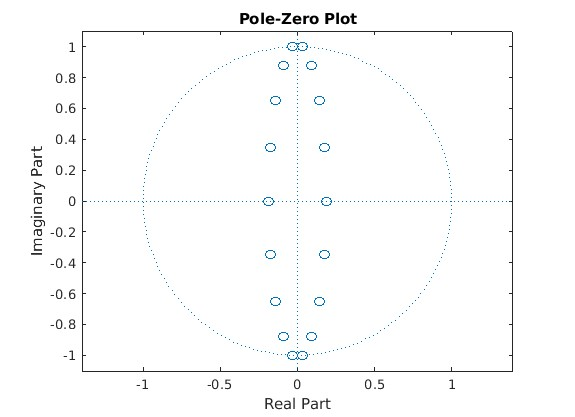
\includegraphics[scale = 0.5]{root_bpf.jpg}
    \caption{}
    \label{fig:my_label}
\end{figure}
In order to get a stable Analog Low Pass Filter we include the poles lying in the Left Half Plane in the Transfer Function. Thus, the required poles are :
        

  

\noindent
\vspace{1em}
\begin{center}
$p_1$ = -0.0322 - 1.0016i \newline
$p_2$ = -0.0927 - 0.8808i  \newline
$p_3$ = -0.1420 - 0.6537i \newline
$p_4$ = -0.0322 + 1.0016i \newline
$p_5$ = -0.0927 + 0.8808i \newline
$p_6$ = -0.1420 + 0.6537i \newline
$p_7$ = -0.1741 - 0.3478i \newline
$p_8$ = -0.1741 + 0.3478i \newline
$p_9$ = -0.1853 + 0.0000i  \newline
\end{center}
\noindent
\vspace{1em}
Using the above poles and the fact that N is odd (no need to normalize by a factor of $\sqrt{1 + D_1}$) i.e. the DC gain is just the product of poles, we can write the analog low pass transfer function as :
\begin{equation*}
    H_{analog}(s) = \frac{\Pi_{i=1}^{9} p_i}{\Pi_{i=1}^{9} (s - p_i)}
\end{equation*}


The values of the coefficients of the corresponding Analog Lowpass Transfer Function  is given as
\begin{table}[H]
    % Center the table
    \centering
    \begin{adjustwidth}{+0cm}{}
        \caption{Denominator Coefficients}
        \begin{tabular}{|c|c|c|c|c|c|c|c|}
            \hline
            Degree & Coefficient & Degree & Coefficient & Degree & Coefficient\\
            \hline
            $s_L^{9}$ & $1.0000 \times 10^{0}$ & $s_L^{8}$ & $1.0672 \times 10^{0}$ & $s_L^{7}$ & $2.8194 \times 10^{0}$ \\
            \hline
            $s_L^{6}$ & $2.2400 \times 10^{0}$ & $s_L^{5}$ & $2.6346 \times 10^{0}$ & $s_L^{4}$ & $1.4660 \times 10^{0}$ \\
            \hline
            $s_L^{3}$ & $0.9108 \times 10^{0}$ & $s_L^{2}$ & $0.3058 \times 10^{0}$ & $s_L^{1}$ & $0.0853 \times 10^{0}$ \\
            \hline
            $s_L^{0}$ & $0.9460099 \times 10^{0}$ & - & -& -&- \\
            \hline
        \end{tabular}
    \end{adjustwidth}
\end{table}
\subsubsection{Analog Bandpass Transfer Function}
The transformation is given by :
\begin{equation*}
    s_L = \frac{s^2 + \Omega_o^2 }{Bs}
\end{equation*}
Substituting the values of B and $\Omega_o$
\begin{equation*}
    s_L = \frac{s^2 + 0.8949}{3.492s}
\end{equation*}
After substituting it can be written in the form N(s)/D(s) where the coefficients of N(s) and D(s) are given below :

\begin{equation*}
    N(s) = 763.1035. s^{9} 
\end{equation*}


\begin{table}[H]
    % Center the table
    \centering
    \begin{adjustwidth}{+0cm}{}
        \caption{Denominator Coefficients}
        \begin{tabular}{|c|c|c|c|c|c|c|c|}
            \hline
            Degree & Coefficient & Degree & Coefficient & Degree & Coefficient\\
            \hline
            $s^{18}$ & $1.0000$ & $s^{17}$ & $3.7265$ & $s^{16}$ & $42.4344$ \\
            \hline
            $s^{15}$ & $122.0610$ & $s^{14}$ & $635.9561$ & $s^{13}$ & $1356.9490$ \\
            \hline
            $s^{12}$ & $4042.8322$ & $s^{11}$ & $5956.3007$ & $s^{10}$ & $10400.9982$ \\
            \hline
            $s^{9}$ & $9420.5746$ & $s^{8}$ & $9308.0197$ & $s^{7}$ & $4770.2502$ \\
            \hline
            $s^{6}$ & $2897.5607$ & $s^{5}$ & $870.3474$ & $s^{4}$ & $365.0383$ \\
            \hline
            $s^{3}$ & $62.7005$ & $s^{2}$ & $19.5071$ & $s^{1}$ & $1.5331$ \\
            \hline
            $s^{0}$ & $0.3682$ & - & - & - & - \\
            \hline
        \end{tabular}
    \end{adjustwidth}
\end{table}

\subsubsection{Discrete Time Filter Transfer Function}
To transform the analog domain transfer function into the discrete domain, we need to make use ofthe Bilinear Transformation which is given as :
\begin{equation*}
    s = \frac{1 - z^{-1}}{1 + z^{-1}}
\end{equation*}
Using  above  equation  we  get $H_{discrete,BPF}$(z)  from $H_{analog,BPF}$(s).It  can  be  written  in  the  form N(z)/D(z) where the coefficients of the polynomials N(z) and D(z) are given as :-

\begin{table}[H]
    % Center the table
    \centering
    \caption{Numerator Coefficients}
    \begin{tabular}{|c|c|c|c|c|c|c|c|}
        \hline
        \textbf{Degree} & \textbf{Coefficient} & \textbf{Degree} & \textbf{Coefficient} & \textbf{Degree} & \textbf{Coefficient}\\
        \hline
        $s^{18}$ & $0.0152$ & $s^{17}$ & $0$ & $s^{16}$ & $-0.1366$ \\
        \hline
        $s^{15}$ & $0$ & $s^{14}$ & $0.5464$ & $s^{13}$ & $0$ \\
        \hline
        $s^{12}$ & $-1.2749$ & $s^{11}$ & $0$ & $s^{10}$ & $1.9124$ \\
        \hline
        $s^{9}$ & $0$ & $s^{8}$ & $-1.9124$ & $s^{7}$ & $0$ \\
        \hline
        $s^{6}$ & $1.2749$ & $s^{5}$ & $0$ & $s^{4}$ & $-0.5464$ \\
        \hline
        $s^{3}$ & $0$ & $s^{2}$ & $0.1366$ & $s^{1}$ & $0$ \\
        \hline
        $s^{0}$ & $-0.0152$ & - & - & - & - \\
        \hline
    \end{tabular}
\end{table}


\begin{table}[H]
        % Center the table
    \centering
    \begin{adjustwidth}{+0cm}{}
    \caption{Denominator Coefficients}
    \begin{tabular}{|c|c|c|c|c|c|c|c|}
        \hline
        Degree & Coefficient & Degree & Coefficient & Degree & Coefficient\\
        \hline
        $s^{18}$ & $1.0000$ & $s^{17}$ & $-0.4273$ & $s^{16}$ & $-1.2084$ \\
        \hline
        $s^{15}$ & $0.2881$ & $s^{14}$ & $2.4685$ & $s^{13}$ & $-0.7523$ \\
        \hline
        $s^{12}$ & $-1.1718$ & $s^{11}$ & $0.0748$ & $s^{10}$ & $1.5745$ \\
        \hline
        $s^{9}$ & $-0.4211$ & $s^{8}$ & $0.0169$ & $s^{7}$ & $-0.1342$ \\
        \hline
        $s^{6}$ & $0.4522$ & $s^{5}$ & $-0.1686$ & $s^{4}$ & $0.2671$ \\
        \hline
        $s^{3}$ & $-0.0526$ & $s^{2}$ & $0.0653$ & $s^{1}$ & $-0.0540$ \\
        \hline
        $s^{0}$ & $0.1024$ & - & - & - & - \\
        \hline
\end{tabular}
\end{adjustwidth}
\end{table}

\subsubsection{Matlab Plots}
\textbf{Magmitude Response}
\begin{figure}[H]
\hspace*{-2.5cm}
    \centering
    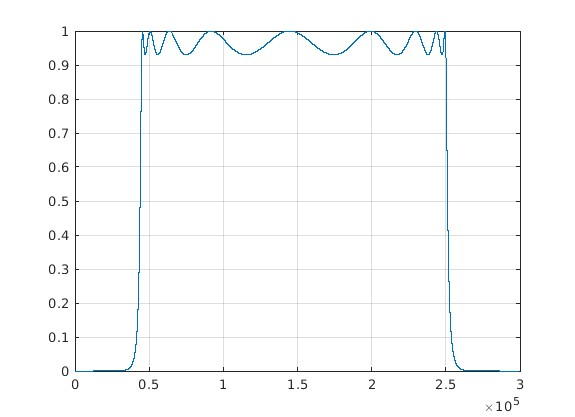
\includegraphics[scale = 0.5]{bpf_cheby_mag.jpg}
    \label{fig:my_label}
\end{figure}

\textbf{Frequency Response}
\begin{figure}[H]
\hspace*{-2.5cm}
    \centering
    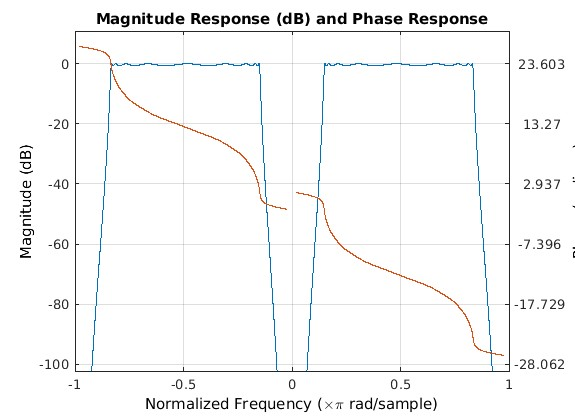
\includegraphics[scale = 0.5]{bpf_cheby_magphase.jpg}
    \label{fig:my_label}
\end{figure}

\textbf{Pole - Zero Plot}
\begin{figure}[H]
\hspace*{-2.5cm}
    \centering
    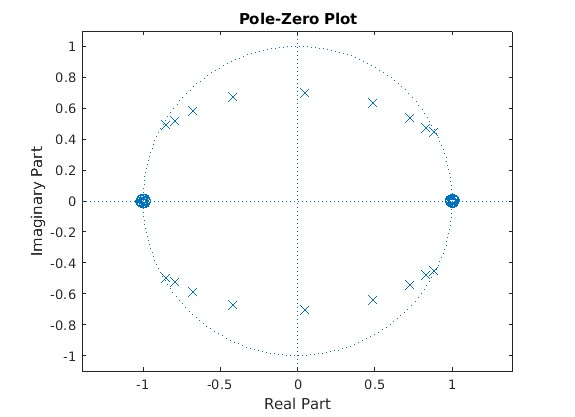
\includegraphics[scale = 0.5]{polezero_bpf.jpg}
    \label{fig:my_label}
\end{figure}


\textbf{Unnormalized Phase response}
\begin{figure}[H]
\hspace*{-2.5cm}
    \centering
    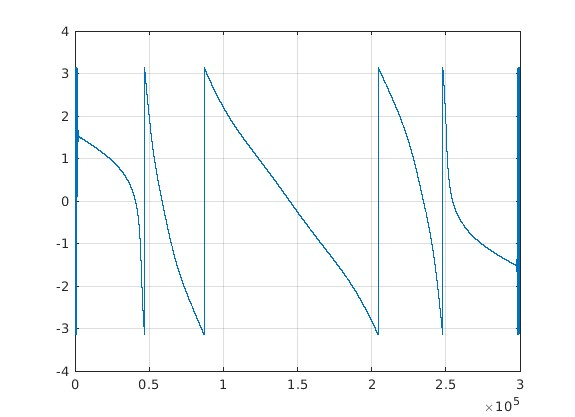
\includegraphics[scale = 0.5]{bpf_cheby_phase.jpg}
    \label{fig:my_label}
\end{figure}

\subsection{\textbf{Bandstop Chebyshev Filter}}
\subsubsection{\textbf{Un-normalized Discrete Time Filter Specifications}}

\noindent
The specifications of this filter are :
\begin{itemize}
    \item Stopband : \textbf{80 - 215 KHz}
    \item Passband : \textbf{0 - 75 KHz} and \textbf{220 - 300 KHz}
    \item  Transition band : \textbf{5KHz} on either side of passband
    \item  Tolerance : \textbf{0.07} in \textbf{magnitude} for both passband and stopband
    \item  Nature : Passbands are \textbf{oscillatory} and stopbands are \textbf{monotonic}
\end{itemize}

\subsubsection{Normalized Digital Filter Specifications}

In the normalized frequency axis, sampling rate corresponds to 2$\pi$\\
Therefore, any frequency can be normalized as follows :
\begin{equation*}
    \omega = \frac{\Omega*2\pi}{\Omega_s}
\end{equation*}
where $\Omega_s$ is the Sampling Rate.\\

\vspace{1em}
\noindent
For the normalized discrete filter specifications, the nature and tolerances being the dependent variables remain the same while the passband and stopband frequencies change as per the above transformations. 
\begin{itemize}
    \item Stopband : \textbf{0.267 - 0.717} {$\pi$}
    \item Passband : \textbf{0 -  0.25} {$\pi$} and \textbf{0.733 - 1} {$\pi$}
    \item  Transition band : \textbf{0.0167} $\pi$ on either side of stopband
\end{itemize}

\subsubsection{Bilinear Transformation}
To convert to analog domain, we use the following bilinear transformation :
\begin{equation*}
    s = \frac{1 - z^{-1}}{1 + z^{-1}}
\end{equation*}
\begin{equation*}
    \Omega_{analog} = \tan (\frac{w}{2})
\end{equation*}
Applying the transformation at Band Edges we get :
\begin{table}[H]
		% Center the table
		\begin{center}
		\begin{tabular}{|c|c|}
			% To create a horizontal line, type \hline
			\hline
			% To end a column type &
			% For a linebreak type \\
			$\omega$ & $\Omega$\\
			
			\hline
                0 & 0\\
                \hline
                0.25 $\pi$ & 0.414 \\
                \hline
                0.267 $\pi$ & 0.445\\
                \hline
                0.717 $\pi$ & 2.097\\
                \hline
                0.733 $\pi$ & 2.246\\
                \hline
                $\pi$ & $\infty$\\
                \hline
            
		\end{tabular}
		\end{center}
\end{table}

Therefore, the corresponding specifications are :
\begin{itemize}
    \item Stopband :  \textbf{0.445} ($\Omega_{s1}$) - \textbf{2.097} ($\Omega_{s2}$)
    \item  Transition band : Between the passband and stopband edges
    \item Passband : \textbf{0 - 0.414}($\Omega_{p1}$) and \textbf{2.246} ($\Omega_{p2}$) \textbf{- $\infty$}
\end{itemize}

\subsubsection{Frequency Transformation and Relevant Parameters}
We need to convert the Band - Stop filter into a Low - Pass analog filter as we are aware of it's frequency response. For that purpose we use the following frequency transformation with two parameters B and $\Omega_o$

\begin{equation*}
    \Omega_l = \frac{B\Omega}{ \Omega_o^2 - \Omega^2}
\end{equation*}

\vspace{1em}
\noindent
If we follow the convention that the passband edges are mapped to +1 and -1, the parameters, in terms of the passband edges can be obtained by solving two equations and are given by :
\begin{equation*}
    \Omega_o = \sqrt{\Omega_{p1} \Omega_{p2}} = \sqrt{0.414*2.246} = 0.964
\end{equation*}
\begin{equation*}
    B = \Omega_{p2}  - \Omega_{p1} = 1.832
\end{equation*}

\begin{table}[H]
		% Center the table
		\begin{center}
		\begin{tabular}{|c|c|}
			% To create a horizontal line, type \hline
			\hline
			% To end a column type &
			% For a linebreak type \\
			$\Omega$ & $\Omega_L$\\
			
			\hline
                $0^{+}$ & $0^{+}$\\
                \hline
                0.414 ($\Omega_{p1}$) & +1 \\
                \hline
                0.445 ($\Omega_{s1}$) & 1.115\\
                \hline
                $0.946^{-}$ ($\Omega_o$) & $\infty$\\
                \hline
                $0.946^{+}$ ($\Omega_o$) & $-\infty$\\
                \hline
                2.097 ($\Omega_{s2}$)  & -1.108\\
                \hline
                2.246 ($\Omega_{p2}$) & -1\\
                \hline
                $\infty$ & $0^{-}$\\
                \hline
            
		\end{tabular}
		\end{center}
\end{table}

\vspace{1em}
\noindent
To make the filter as close to ideal as possible we choose the more stringent stopband for the lowpass filter i.e. $\Omega_{sL}$ = min($\Omega_{sL1}$ , - $\Omega_{sL2}$) = 1.108. (where $\Omega_{sL}$ stands for the stopband for the lowpass filter)

\vspace{1em}
\noindent
Therefore the analog lowpass filter specifications are as follows:
\begin{itemize}
    \item Passband Edge : 1 ($\Omega_{pL}$)
    \item Stopband Edge : 1.108 ($\Omega_{sL}$)
\end{itemize}

\subsubsection{Analog Lowpass Transfer Function}
To keep the frequency response monotonic in passband and stopband we use the Chebyshev approximation and let the transfer function of the analog lowpass filter to be of the form : 

\begin{equation*}
    |H(j\Omega)|^2 = \frac{1}{1 + \epsilon^2C^2_{N}(\frac{\Omega}{\Omega_p})}
\end{equation*}

where $\Omega_p = 1$ and $C_N$ is the Chebyschev Polynomial given by

\begin{equation*}
    C_N(\Omega) = cos(Ncos^{-1}(\Omega))
\end{equation*}

\vspace{1em}
\noindent
We define two new parameters $D_1$ and $D_2$ such that
\begin{equation*}
    D_1 = \frac{1}{(1 - \delta_1)^2} - 1 = 0.1562
\end{equation*}
\begin{equation}
    D_2 = \frac{1}{(\delta_2)^2} - 1 = 203.0816
\end{equation}
where $\delta_1$ = $\delta_2$ = 0.07

\vspace{1em}
\noindent
We choose $\epsilon$ of the Chebyschev Filter to be $\sqrt{D_1}$ (to minimize N) and then upon applying the condition that the stopband must lie within the tolerances specified, we get a lower bound on the value of N which is given by:
\begin{equation*}
    N = \left\lceil   \frac{\cosh^{-1}(\sqrt{\frac{D_2}{D_1}})}{\cosh^{-1}(\frac{\Omega_s}{\Omega_p})} \right\rceil = 10
\end{equation*}
The poles of the transfer function can be obtained by solving the equation
\begin{equation*}
    1 + D_1\cosh^2(N\cosh^{-1}(\frac{s}{j})) = 0
\end{equation*}
which is nothing but
\begin{equation*}
    1 + 0.1562(C^2_10(s/j)) = 0
\end{equation*}
where $C_{10}(x) = 512x^{10} - 1280x^8 + 1120x^6 - 400x^4 + 50x^2 - 1$ 

Using MATLAB, we plot the poles of the magnitude response of the analog low pass filter.
\begin{figure}[H]
    \centering
    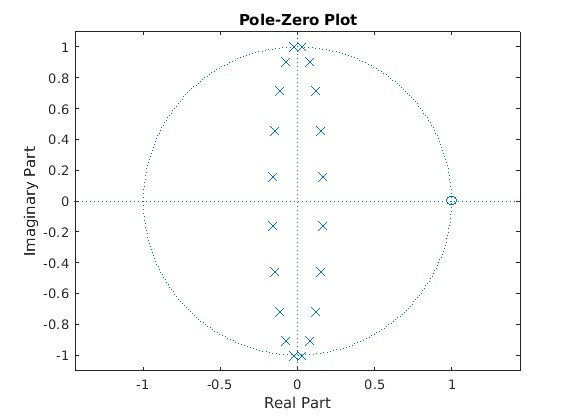
\includegraphics[scale = 0.5]{root_bsf.jpg}
    \caption{}
    \label{fig:my_label}
\end{figure}
In order to get a stable Analog Low Pass Filter we include the poles lying in the Left Half Plane in the Transfer Function. Thus, the required poles are :
        

\noindent
\vspace{1em}
\begin{center}
$p_{ 1 }$ =  -0.0261  + j 1.0013 \\
$p_{ 2 }$ =  -0.0756  + j 0.9033 \\
$p_{ 3 }$ =  -0.1178  + j 0.7169 \\
$p_{ 4 }$ =  -0.1484  + j 0.4602 \\
$p_{ 5 }$ =  -0.0261  - j 1.0013 \\
$p_{ 6 }$ =  -0.0756  - j 0.9033 \\
$p_{ 7 }$ =  -0.1178  - j 0.7169 \\
$p_{ 8 }$ =  -0.1484  - j 0.4602 \\
$p_{ 9 }$ =  -0.1645  + j 0.1586 \\
$p_{ 10 }$ =  -0.1645  - j 0.1586 \\
\end{center}
\noindent
\vspace{1em}
Using the above poles and the fact that N is even (we need to normalize by a factor of $\sqrt{1 + D_1}$) i.e. the DC gain is just the product of poles times $\sqrt{1 + D_1}$, we can write the analog low pass transfer function as :
\begin{equation*}
        H_{\text{analog}}(s) = \frac{\prod_{i=1}^{11} p_i}{\sqrt{1 + D_1} \prod_{i=1}^{11} (s - p_i)}
\end{equation*}
The values of the coefficients of the corresponding Analog Lowpass Transfer Function  is given as
\begin{table}[H]
        % Center the table
  \centering
        \begin{adjustwidth}{-2.5cm}{}
        \caption{Denominator Coefficients}
        \begin{tabular}{|c|c|c|c|c|c|c|c|c|c|c|c|}
\hline
Degree & Coefficient & Degree & Coefficient & Degree & Coefficient & Degree & Coefficient & Degree & Coefficient\\
\hline
$s_L^{10}$ & $1.0650$ & $s_L^9$ & $3.0671$ & $s_L^8$ & $2.5024$ & $s_L^7$ & $3.2740$ & $s_L^6$ & $1.9568$ \\
\hline
$s_L^5$ & $1.4234$ & $s_L^4$ & $0.5652$ & $s_L^3$ & $0.2169$ & $s_L^2$ & $0.0439$ & $s_L^1$ & $0.0053$ \\
\hline
  	\end{tabular}
    \end{adjustwidth}
\end{table}

\subsubsection{Analog Bandstop Transfer Function}
The transformation is given by :
\begin{equation*}
    s_L = \frac{Bs}{s^2 + \Omega_o^2 }
\end{equation*}
Substituting the values of B and $\Omega_o$
\begin{equation*}
    s_L = \frac{1.832s}{s^2 + 0.9293}
\end{equation*}
After substituting it can be written in the form N(s)/D(s) where the coefficients of N(s) and D(s) are given below :

\begin{table}[H]
      % Center the table
  \centering
      \begin{adjustwidth}{-2.5cm}{}
      \caption{Numerator Coefficients}
      \begin{tabular}{|c|c|c|c|c|c|c|c|c|c|c|c|}
\hline
Degree & Coefficient & Degree & Coefficient & Degree & Coefficient & Degree & Coefficient & Degree & Coefficient\\
\hline
$s^{ 20 }$ & $ 0.9300 $ & $s^{ 18 }$ & $ 8.6425 $ & $s^{ 16 }$ & $ 36.1413 $  & $s^{ 14 }$ & $ 89.5625 $ & $s^{ 12 }$ & $ 145.6527 $ \\
\hline
$s^{ 10 }$ & $ 162.4254 $ & $s^{ 8 }$ & $ 125.7844 $ & $s^{ 6 }$ & $ 66.7948 $  & $s^{ 4 }$ & $ 23.2771 $ & $s^{ 2 }$ & $ 4.8069 $ \\
\hline
$s^{ 0 }$ & $ 0.4467 $ & - & - & - & - & - & - & - & - \\
\hline
  	\end{tabular}
    \end{adjustwidth}
\end{table}


\begin{table}[H]
    % Center the table
    \centering
    \begin{adjustwidth}{0cm}{}
        \caption{Denominator Coefficients}
        \begin{tabular}{|c|c|c|c|c|c|}
            \hline
            Degree & Coefficient & Degree & Coefficient & Degree & Coefficient \\
            \hline
            $s^{20}$ & $1.0$ & $s^{19}$ & $15.1199$ & $s^{18}$ & $146.2702$ \\
            \hline
            $s^{17}$ & $780.4144$ & $s^{16}$ & $4074.5577$ & $s^{15}$ & $12323.4978$ \\
            \hline
            $s^{14}$ & $43525.5871$ & $s^{13}$ & $80805.5406$ & $s^{12}$ & $205220.0782$ \\
            \hline
            $s^{11}$ & $222934.7104$ & $s^{10}$ & $392707.4681$ & $s^{9}$ & $207172.3347$ \\
            \hline
            $s^{8}$ & $177226.2239$ & $s^{7}$ & $64849.0090$ & $s^{6}$ & $32460.9263$ \\
            \hline
            $s^{5}$ & $8540.9137$ & $s^{4}$ & $2624.2480$ & $s^{3}$ & $467.0934$ \\
            \hline
            $s^{2}$ & $81.3558$ & $s^{1}$ & $7.8151$ & $s^{0}$ & $0.4803$ \\
            \hline
        \end{tabular}
    \end{adjustwidth}
\end{table}

\subsubsection{Discrete Time Filter Transfer Function}
To transform the analog domain transfer function into the discrete domain, we need to make use ofthe Bilinear Transformation which is given as :
\begin{equation*}
    s = \frac{1 - z^{-1}}{1 + z^{-1}}
\end{equation*}
Using  above  equation  we  get $H_{discrete,BSF}$(z)  from $H_{analog,BSF}$(s).It  can  be  written  in  the  form N(z)/D(z) where the coefficients of the polynomials N(z) and D(z) are given as :-

\begin{table}[H]
    % Center the table
    \centering
    \begin{adjustwidth}{0cm}{}
    \caption{Numerator Coefficients}
    \begin{tabular}{|c|c|c|c|c|c|}
        \hline
        Degree & Coefficient & Degree & Coefficient & Degree & Coefficient \\
        \hline
        $s^{20}$ & $4.5637 \times 10^{-4}$ & $s^{19}$ & $-3.3449 \times 10^{-4}$ & $s^{18}$ & $4.6741 \times 10^{-3}$ \\
        \hline
        $s^{17}$ & $-3.0321 \times 10^{-3}$ & $s^{16}$ & $2.1422 \times 10^{-2}$ & $s^{15}$ & $-1.2193 \times 10^{-2}$ \\
        \hline
        $s^{14}$ & $5.7871 \times 10^{-2}$ & $s^{13}$ & $-2.8552 \times 10^{-2}$ & $s^{12}$ & $1.0206 \times 10^{-1}$ \\
        \hline
        $s^{11}$ & $-4.2904 \times 10^{-2}$ & $s^{10}$ & $1.2278 \times 10^{-1}$ & $s^{9}$ & $-4.2904 \times 10^{-2}$ \\
        \hline
        $s^{8}$ & $1.0206 \times 10^{-1}$ & $s^{7}$ & $-2.8552 \times 10^{-2}$ & $s^{6}$ & $5.7871 \times 10^{-2}$ \\
        \hline
        $s^{5}$ & $-1.2193 \times 10^{-2}$ & $s^{4}$ & $2.1422 \times 10^{-2}$ & $s^{3}$ & $-3.0321 \times 10^{-3}$ \\
        \hline
        $s^{2}$ & $4.6741 \times 10^{-3}$ & $s^{1}$ & $-3.3449 \times 10^{-4}$ & $s^{0}$ & $4.5637 \times 10^{-4}$ \\
        \hline
    \end{tabular}
    \end{adjustwidth}
\end{table}


\begin{table}[H]
    % Center the table
    \centering
    \begin{adjustwidth}{0cm}{}
        \caption{Denominator Coefficients}
        \begin{tabular}{|c|c|c|c|c|c|}
            \hline
            Degree & Coefficient & Degree & Coefficient & Degree & Coefficient \\
            \hline
            $s^{20}$ & $1.0$ & $s^{19}$ & $-0.2669$ & $s^{18}$ & $-2.6825$ \\
            \hline
            $s^{17}$ & $0.4631$ & $s^{16}$ & $5.8313$ & $s^{15}$ & $-0.7486$ \\
            \hline
            $s^{14}$ & $-8.7725$ & $s^{13}$ & $0.6917$ & $s^{12}$ & $10.6737$ \\
            \hline
            $s^{11}$ & $-0.4520$ & $s^{10}$ & $-10.3559$ & $s^{9}$ & $0.1059$ \\
            \hline
            $s^{8}$ & $8.1526$ & $s^{7}$ & $0.1181$ & $s^{6}$ & $-5.1175$ \\
            \hline
            $s^{5}$ & $-0.1661$ & $s^{4}$ & $2.4837$ & $s^{3}$ & $0.1015$ \\
            \hline
            $s^{2}$ & $-0.8586$ & $s^{1}$ & $-0.0339$ & $s^{0}$ & $0.1787$ \\
            \hline
        \end{tabular}
    \end{adjustwidth}
\end{table}
\newpage
\subsubsection{Matlab Plots}
\textbf{Magnitude Response}
\begin{figure}[H]
\hspace*{-2.5cm}
    \centering
    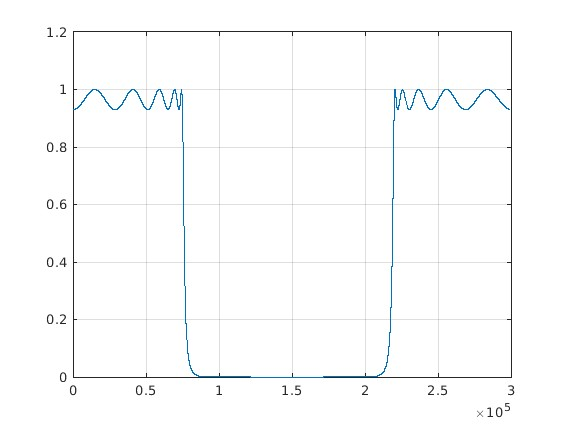
\includegraphics[scale = 0.5]{bsf_cheby_mag.jpg}
    \label{fig:my_label}
\end{figure}

\textbf{Frequency Response}
\begin{figure}[H]
\hspace*{-2.5cm}
    \centering
    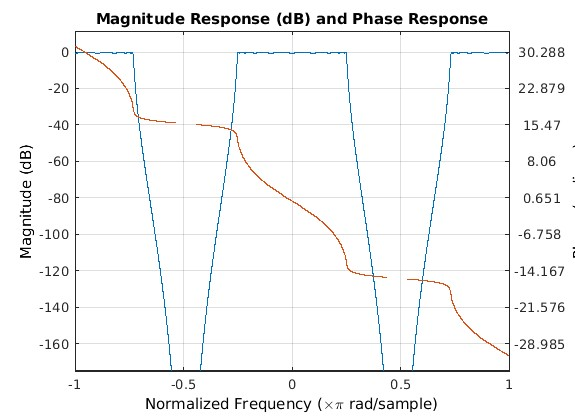
\includegraphics[scale = 0.5]{bsf_cheby_magphase.jpg}
    \label{fig:my_label}
\end{figure}

\textbf{Pole - Zero Plot}
\begin{figure}[H]
\hspace*{-2.5cm}
    \centering
    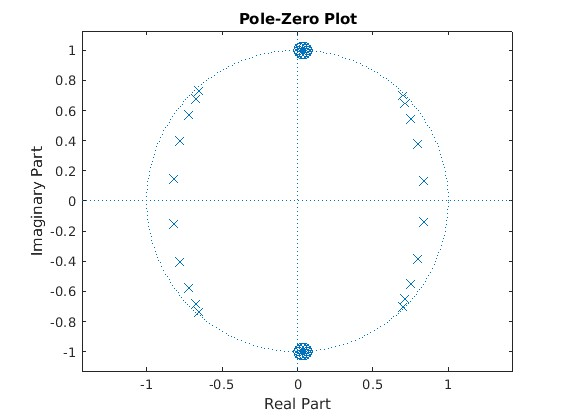
\includegraphics[scale = 0.5]{polezero_bsf.jpg}
    \label{fig:my_label}
\end{figure}

\textbf{Unnormalized Phase response}
\begin{figure}[H]
\hspace*{-2.5cm}
    \centering
    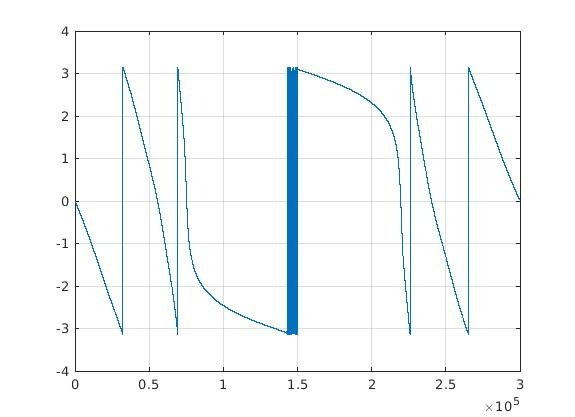
\includegraphics[scale = 0.5]{bsf_cheby_phase.jpg}
    \label{fig:my_label}
\end{figure}

\subsection{Final Results}
Using the above two designed Chebyschev filters, we can cascade them to get the desired Multiband IIR Filter. The resulting polynomial will have a degree of 20. The coefficients of the numerator and denominator of the transfer function are given below :
\begin{table}[H]
    % Center the table
    \centering
    \begin{adjustwidth}{0cm}{}
        \caption{Numerator Coefficients}
        \begin{tabular}{|c|c|c|c|c|c|}
            \hline
            Degree & Coefficient & Degree & Coefficient & Degree & Coefficient \\
            \hline
            $s^{38}$ & $6.9267 \times 10^{-6}$ & $s^{37}$ & $-5.0769 \times 10^{-6}$ & $s^{36}$ & $8.6012 \times 10^{-6}$ \\
            \hline
            $s^{35}$ & $-3.2729 \times 10^{-7}$ & $s^{34}$ & $-6.3973 \times 10^{-5}$ & $s^{33}$ & $4.6343 \times 10^{-5}$ \\
            \hline
            $s^{32}$ & $-7.5862 \times 10^{-5}$ & $s^{31}$ & $1.9785 \times 10^{-6}$ & $s^{30}$ & $0.0003$ \\
            \hline
            $s^{29}$ & $-0.0002$ & $s^{28}$ & $0.0003$ & $s^{27}$ & $-4.6412 \times 10^{-6}$ \\
            \hline
            $s^{26}$ & $-0.0006$ & $s^{25}$ & $0.0004$ & $s^{24}$ & $-0.0007$ \\
            \hline
            $s^{23}$ & $4.6561 \times 10^{-6}$ & $s^{22}$ & $0.001$ & $s^{21}$ & $-0.0007$ \\
            \hline
            $s^{20}$ & $0.001$ & $s^{19}$ & $-8.8752 \times 10^{-19}$ & $s^{18}$ & $-0.001$ \\
            \hline
            $s^{17}$ & $0.0007$ & $s^{16}$ & $-0.001$ & $s^{15}$ & $-4.6561 \times 10^{-6}$ \\
            \hline
            $s^{14}$ & $0.0007$ & $s^{13}$ & $-0.0004$ & $s^{12}$ & $0.0006$ \\
            \hline
            $s^{11}$ & $4.6412 \times 10^{-6}$ & $s^{10}$ & $-0.0003$ & $s^{9}$ & $0.0002$ \\
            \hline
            $s^{8}$ & $-0.0003$ & $s^{7}$ & $-1.9785 \times 10^{-6}$ & $s^{6}$ & $7.5862 \times 10^{-5}$ \\
            \hline
            $s^{5}$ & $-4.6343 \times 10^{-5}$ & $s^{4}$ & $6.3973 \times 10^{-5}$ & $s^{3}$ & $3.2729 \times 10^{-7}$ \\
            \hline
            $s^{2}$ & $-8.6012 \times 10^{-6}$ & $s^{1}$ & $5.0769 \times 10^{-6}$ & $s^{0}$ & $-6.9267 \times 10^{-6}$ \\
            \hline
        \end{tabular}
    \end{adjustwidth}
\end{table}

\begin{table}[H]

    % Center the table
    \centering
    \begin{adjustwidth}{0cm}{}
        \caption{Denominator Coefficients}
        \begin{tabular}{|c|c|c|c|c|c|}
            \hline
            Degree & Coefficient & Degree & Coefficient & Degree & Coefficient \\
            \hline
            $s^{38}$ & $1$ & $s^{37}$ & $-0.6942$ & $s^{36}$ & $-3.7768$ \\
            \hline
            $s^{35}$ & $2.2198$ & $s^{34}$ & $11.2665$ & $s^{33}$ & $-5.9837$ \\
            \hline
            $s^{32}$ & $-22.9583$ & $s^{31}$ & $10.5732$ & $s^{30}$ & $39.5070$ \\
            \hline
            $s^{29}$ & $-16.1950$ & $s^{28}$ & $-54.8458$ & $s^{27}$ & $19.4920$ \\
            \hline
            $s^{26}$ & $65.9713$ & $s^{25}$ & $-20.6442$ & $s^{24}$ & $-67.0297$ \\
            \hline
            $s^{23}$ & $18.1318$ & $s^{22}$ & $59.3070$ & $s^{21}$ & $-14.1186$ \\
            \hline
            $s^{20}$ & $-44.6107$ & $s^{19}$ & $9.3569$ & $s^{18}$ & $28.6854$ \\
            \hline
            $s^{17}$ & $-5.6179$ & $s^{16}$ & $-15.0545$ & $s^{15}$ & $3.0354$ \\
            \hline
            $s^{14}$ & $6.0454$ & $s^{13}$ & $-1.6439$ & $s^{12}$ & $-1.2623$ \\
            \hline
            $s^{11}$ & $0.9000$ & $s^{10}$ & $-0.4888$ & $s^{9}$ & $-0.5303$ \\
            \hline
            $s^{8}$ & $0.7690$ & $s^{7}$ & $0.2795$ & $s^{6}$ & $-0.5012$ \\
            \hline
            $s^{5}$ & $-0.1385$ & $s^{4}$ & $0.2424$ & $s^{3}$ & $0.0451$ \\
            \hline
            $s^{2}$ & $-0.0744$ & $s^{1}$ & $-0.0131$ & $s^{0}$ & $0.0183$ \\
            \hline
        \end{tabular}
    \end{adjustwidth}
\end{table}


The results of the cascaded Filters are as follows
\subsubsection{Matlab Plots}
\textbf{Frequency Response}
\begin{figure}[H]
\hspace*{-2.5cm}
    \centering
    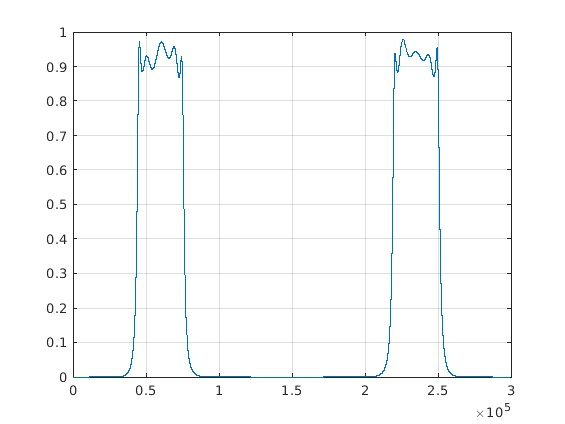
\includegraphics[scale = 0.5]{multiband_cheby_mag.jpg}
    \label{fig:my_label}
\end{figure}

\textbf{Magnitude Response}


\begin{figure}[H]
        \hspace*{-2.5cm}
        \centering
         % Add a valid length value here
        % \hspace{1pt} % Add a valid length value here
        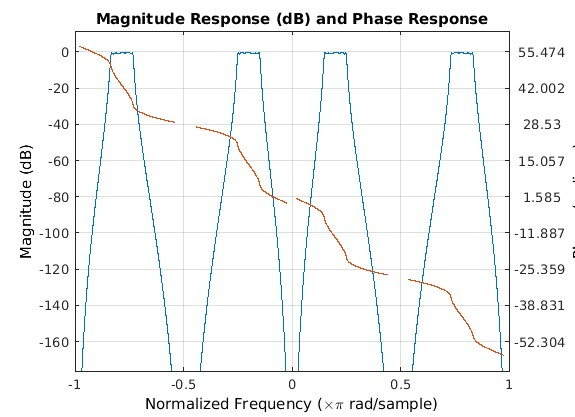
\includegraphics[scale = 0.5]{multiband_cheby_magphase.jpg}
        \caption{}\label{fig:my_label1} % Add caption and label here

    \end{figure}
    
    \textbf{Pole - Zero Plot}
    \begin{figure}[H]
    \hspace*{-2.5cm}
        \centering
        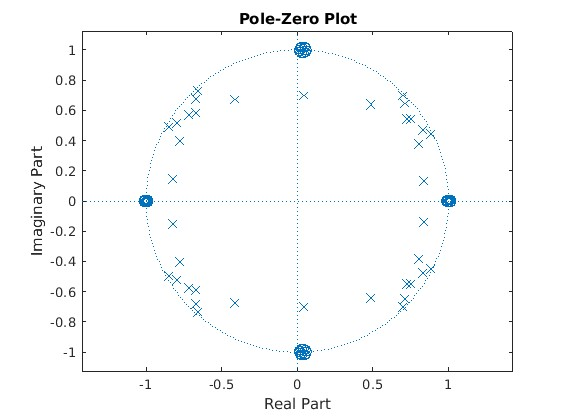
\includegraphics[scale = 0.5]{polezero_final_cheby.jpg}
        \caption{}\label{fig:my_label2} % Add caption and label here
    \end{figure}

    \textbf{Unnormalized Phase response}
\begin{figure}[H]
\hspace*{-2.5cm}
    \centering
    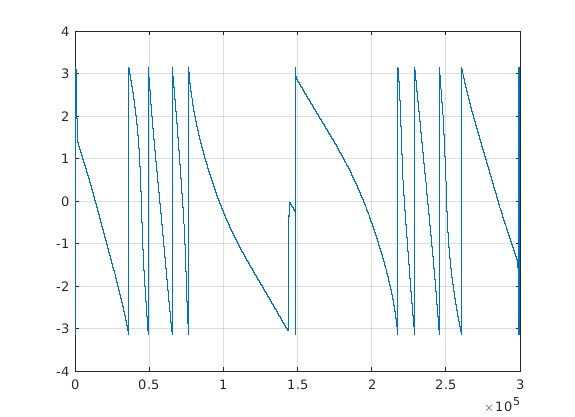
\includegraphics[scale = 0.5]{multiband_cheby_phase.jpg}
    \label{fig:my_label}
\end{figure}
    
\end{document}
% Remove the \end{document} command